% Source: Graph_ML/Graph_AE/graph_autoencoders_tutorial.tex
\begin{notechapter}
% ---- chapter-local definitions ----
\forgetcs\R\newcommand{\R}{\mathbb{R}}
\forgetcs\norm\newcommand{\norm}[1]{\left\|#1\right\|}
\forgetcs\hadamard\newcommand{\hadamard}{\odot}
% -----------------------------------
\chapter{Graph Autoencoders}\label{ch:graph-autoencoders}

\begin{abstract}
This document provides a comprehensive introduction to Graph Autoencoders, focusing on the mathematical foundations of the loss functions used in Structural Deep Network Embedding (SDNE). We develop the intuition behind why standard autoencoder approaches fail for graph structures, and explain in detail how the combined loss function addresses these challenges. Multiple concrete examples illustrate the mathematical concepts.
\end{abstract}

\section{Introduction}

Graph autoencoders extend the classical autoencoder framework to handle graph-structured data. While the encoder-decoder architecture remains conceptually similar, the design of appropriate loss functions requires careful consideration of the unique properties of graph structures.

\subsection{The Autoencoder Framework}

A classical autoencoder consists of:
\begin{itemize}
    \item \textbf{Encoder}: $f: \R^n \to \R^d$ where $d \ll n$ (dimensionality reduction)
    \item \textbf{Decoder}: $g: \R^d \to \R^n$ (reconstruction)
    \item \textbf{Loss function}: Typically $\mathcal{L} = \norm{x - g(f(x))}^2$ (reconstruction error)
\end{itemize}

The goal is to learn a compressed representation that preserves the essential information in the input.

\subsection{Challenges with Graph Structures}

When applying autoencoders to graphs, several critical issues arise:

\begin{enumerate}
    \item \textbf{Sparsity}: Adjacency matrices are extremely sparse (most entries are 0)
    \item \textbf{Asymmetric information}: Edge presence ($A_{ij} = 1$) is informative, but edge absence ($A_{ij} = 0$) does not necessarily indicate dissimilarity
    \item \textbf{Imbalanced learning}: The model naturally tends to predict 0 everywhere to minimize standard reconstruction error
\end{enumerate}

\begin{tcolorbox}[colback=blue!5!white,colframe=blue!75!black,title=Key Insight]
Standard reconstruction loss treats all errors equally. For sparse graphs, this leads to trivial solutions where the model learns to output all zeros.
\end{tcolorbox}

\section{Graph Proximity Measures}

Before diving into the loss functions, we need to understand two fundamental concepts in graph embedding:

\begin{definition}[First-Order Proximity]
First-order proximity measures the direct connection between two nodes. Nodes that are directly connected by an edge should be close in the embedding space.
\end{definition}

\begin{definition}[Second-Order Proximity]
Second-order proximity measures the similarity of two nodes' neighborhoods. Nodes that have similar neighbors should be close in the embedding space, even if they are not directly connected.
\end{definition}

\begin{example}[Proximity Types]
Consider a simple graph:
\begin{center}
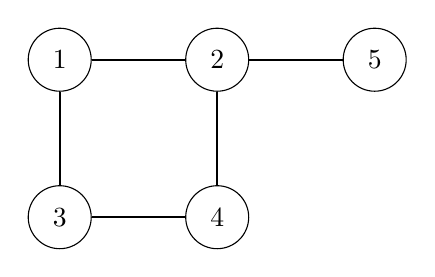
\begin{tikzpicture}[node distance=2cm,
    every node/.style={circle,draw,minimum size=0.8cm}]
    \node (1) {1};
    \node (2) [right of=1] {2};
    \node (3) [below of=1] {3};
    \node (4) [below of=2] {4};
    \node (5) [right of=2] {5};
    
    \draw[thick] (1) -- (2);
    \draw[thick] (1) -- (3);
    \draw[thick] (2) -- (4);
    \draw[thick] (2) -- (5);
    \draw[thick] (3) -- (4);
\end{tikzpicture}
\end{center}

\begin{itemize}
    \item \textbf{First-order}: Nodes 1 and 2 are directly connected, so they should be close
    \item \textbf{Second-order}: Nodes 1 and 5 are not directly connected, but they both connect to node 2, giving them some similarity
\end{itemize}
\end{example}

\section{Loss Function 1: Second-Order Proximity}

\subsection{Mathematical Formulation}

The second-order proximity loss is defined as:
\begin{equation}
\mathcal{L}_{2^{nd}} = \sum_{i} \norm{(\tilde{\bm{A}}_i - \bm{A}_i) \hadamard \bm{B}_i}^2
\label{graph-autoencoders:eq:l2_loss}
\end{equation}

where:
\begin{itemize}
    \item $\bm{A}_i \in \R^n$: The $i$-th row of the adjacency matrix (neighborhood of node $i$)
    \item $\tilde{\bm{A}}_i \in \R^n$: The $i$-th row of the reconstructed adjacency matrix
    \item $\bm{B}_i \in \R^n$: Weight vector with entries:
    \begin{equation}
    B_{ij} = \begin{cases}
    \beta & \text{if } A_{ij} = 1 \\
    1 & \text{if } A_{ij} = 0
    \end{cases}
    \end{equation}
    \item $\hadamard$: Hadamard (element-wise) product
    \item $\beta > 1$: Hyperparameter controlling the penalty for edge reconstruction errors (typically $\beta \in [5, 10]$)
\end{itemize}

\subsection{Intuition Behind the Weighting}

The key innovation is the weight vector $\bm{B}_i$. By setting $B_{ij} = \beta$ when an edge exists, we penalize errors on existing edges much more heavily than errors on non-edges.

\begin{tcolorbox}[colback=green!5!white,colframe=green!75!black,title=Why This Works]
\begin{itemize}
    \item If the model predicts $\tilde{A}_{ij} = 0.1$ when $A_{ij} = 1$, the error $(0.9)^2 \cdot \beta$ is large
    \item If the model predicts $\tilde{A}_{ij} = 0.1$ when $A_{ij} = 0$, the error $(0.1)^2 \cdot 1$ is small
    \item This forces the model to focus on correctly reconstructing existing edges
\end{itemize}
\end{tcolorbox}

\subsection{Detailed Example: Computing $\mathcal{L}_{2^{nd}}$}

\begin{example}[Second-Order Loss Calculation]
Consider a 5-node graph where node $i$ has the following adjacency vector:
\[
\bm{A}_i = [0, 1, 1, 0, 1]
\]
Node $i$ is connected to nodes 2, 3, and 5.

The autoencoder produces a reconstruction:
\[
\tilde{\bm{A}}_i = [0.1, 0.8, 0.9, 0.05, 0.7]
\]

With $\beta = 5$, the weight vector is:
\[
\bm{B}_i = [1, 5, 5, 1, 5]
\]

\textbf{Step 1}: Compute the reconstruction error:
\[
\bm{A}_i - \tilde{\bm{A}}_i = [-0.1, 0.2, 0.1, -0.05, 0.3]
\]

\textbf{Step 2}: Apply element-wise weighting:
\[
(\bm{A}_i - \tilde{\bm{A}}_i) \hadamard \bm{B}_i = [-0.1, 1.0, 0.5, -0.05, 1.5]
\]

\textbf{Step 3}: Compute squared norm:
\begin{align*}
\mathcal{L}_{2^{nd}}(i) &= \norm{[-0.1, 1.0, 0.5, -0.05, 1.5]}^2 \\
&= (-0.1)^2 + (1.0)^2 + (0.5)^2 + (-0.05)^2 + (1.5)^2 \\
&= 0.01 + 1.0 + 0.25 + 0.0025 + 2.25 \\
&= 3.5125
\end{align*}

\textbf{Comparison without weighting} ($\beta = 1$):
\begin{align*}
\mathcal{L}_{2^{nd}-{unweighted}}(i) &= (-0.1)^2 + (0.2)^2 + (0.1)^2 + (-0.05)^2 + (0.3)^2 \\
&= 0.155
\end{align*}

The weighted version is approximately 22 times larger! This demonstrates how the weighting scheme dramatically increases the penalty for errors on existing edges.
\end{example}

\subsection{Why "Second-Order"?}

The loss function preserves second-order proximity because:

\begin{proposition}
If nodes $i$ and $j$ have similar adjacency vectors ($\bm{A}_i \approx \bm{A}_j$),
then minimizing $\mathcal{L}_{2^{nd}}$ encourages their embeddings to be similar.
\end{proposition}

\begin{proof}[Intuition]
The encoder maps adjacency vectors to embeddings. If $\bm{A}_i \approx \bm{A}_j$, and both are reconstructed accurately, then the encoder must map them to similar embeddings $\bm{y}_i \approx \bm{y}_j$ (otherwise, the decoder could not produce similar outputs from different embeddings).
\end{proof}

\section{Loss Function 2: First-Order Proximity}

\subsection{Mathematical Formulation}

The first-order proximity loss is defined as:
\begin{equation}
\mathcal{L}_{1^{st}} = \sum_{i,j} S_{ij} \norm{\bm{y}_i - \bm{y}_j}^2_2
\label{graph-autoencoders:eq:l1_loss}
\end{equation}

where:
\begin{itemize}
    \item $\bm{y}_i, \bm{y}_j \in \R^d$: Embedding vectors for nodes $i$ and $j$ (output of encoder)
    \item $S_{ij}$: Strength/weight of the connection between nodes $i$ and $j$
    \item For unweighted graphs: $S_{ij} = A_{ij} \in \{0, 1\}$
    \item For weighted graphs: $S_{ij}$ is the edge weight
\end{itemize}

\subsection{Intuition Behind First-Order Loss}

The loss function explicitly penalizes distance between embeddings of connected nodes:

\begin{itemize}
    \item If $S_{ij}$ is large (strong connection), then $\norm{\bm{y}_i - \bm{y}_j}^2$ must be small to keep loss low
    \item If $S_{ij} = 0$ (no connection), this term contributes nothing to the loss
    \item Connected nodes are pulled together in embedding space
\end{itemize}

\begin{tcolorbox}[colback=yellow!5!white,colframe=yellow!75!black,title=Geometric Interpretation]
Think of $\mathcal{L}_{1^{st}}$ as a spring system where each edge is a spring pulling connected nodes together. Stronger edges ($S_{ij}$ larger) correspond to stiffer springs.
\end{tcolorbox}

\subsection{Detailed Example: Computing $\mathcal{L}_{1^{st}}$}

\begin{example}[First-Order Loss Calculation]
Consider a simple path graph with 3 nodes: $1 - 2 - 3$

The adjacency matrix is:
\[
\bm{A} = \begin{bmatrix}
0 & 1 & 0 \\
1 & 0 & 1 \\
0 & 1 & 0
\end{bmatrix}
\]

Suppose the encoder produces 2D embeddings:
\begin{align*}
\bm{y}_1 &= [0, 0] \\
\bm{y}_2 &= [1, 0] \\
\bm{y}_3 &= [2, 0]
\end{align*}

\textbf{Computing the loss}:

Since $S_{ij} = A_{ij}$, only edges $(1,2)$ and $(2,3)$ contribute:

\begin{align*}
\mathcal{L}_{1^{st}} &= S_{12} \norm{\bm{y}_1 - \bm{y}_2}^2 + S_{23} \norm{\bm{y}_2 - \bm{y}_3}^2 \\
&= 1 \cdot \norm{[0,0] - [1,0]}^2 + 1 \cdot \norm{[1,0] - [2,0]}^2 \\
&= 1 \cdot \norm{[-1,0]}^2 + 1 \cdot \norm{[-1,0]}^2 \\
&= 1 \cdot 1 + 1 \cdot 1 \\
&= 2
\end{align*}

\textbf{Compare with bad embeddings}:

Suppose instead:
\begin{align*}
\bm{y}_1 &= [0, 0] \\
\bm{y}_2 &= [5, 5] \\
\bm{y}_3 &= [10, 10]
\end{align*}

Then:
\begin{align*}
\mathcal{L}_{1^{st}} &= 1 \cdot \norm{[5,5]}^2 + 1 \cdot \norm{[5,5]}^2 \\
&= 1 \cdot 50 + 1 \cdot 50 \\
&= 100
\end{align*}

The poor embeddings result in a loss that is 50 times larger!
\end{example}

\subsection{Expansion of the Loss}

We can expand equation \eqref{graph-autoencoders:eq:l1_loss} to better understand its behavior:

\begin{align}
\mathcal{L}_{1^{st}} &= \sum_{i,j} S_{ij} \norm{\bm{y}_i - \bm{y}_j}^2_2 \nonumber \\
&= \sum_{i,j} S_{ij} (\bm{y}_i - \bm{y}_j)^T(\bm{y}_i - \bm{y}_j) \nonumber \\
&= \sum_{i,j} S_{ij} (\bm{y}_i^T\bm{y}_i - 2\bm{y}_i^T\bm{y}_j + \bm{y}_j^T\bm{y}_j) \nonumber \\
&= \sum_{i,j} S_{ij} (\norm{\bm{y}_i}^2 - 2\bm{y}_i^T\bm{y}_j + \norm{\bm{y}_j}^2)
\label{graph-autoencoders:eq:l1_expanded}
\end{align}

This form shows that the loss:
\begin{itemize}
    \item Encourages the dot product $\bm{y}_i^T\bm{y}_j$ to be large (embeddings aligned)
    \item Is minimized when connected nodes have similar embeddings
\end{itemize}

\section{Combined Loss: SDNE Framework}

\subsection{Complete Formulation}

The Structural Deep Network Embedding (SDNE) framework combines both loss functions with a regularization term:

\begin{equation}
\mathcal{L}_{total} = \mathcal{L}_{2^{nd}} + \alpha \mathcal{L}_{1^{st}} + \lambda \mathcal{L}_{reg}
\label{graph-autoencoders:eq:total_loss}
\end{equation}

where:
\begin{align}
\mathcal{L}_{2^{nd}} &= \sum_{i} \norm{(\tilde{\bm{A}}_i - \bm{A}_i) \hadamard \bm{B}_i}^2 \quad \text{(second-order)} \\
\mathcal{L}_{1^{st}} &= \sum_{i,j} S_{ij} \norm{\bm{y}_i - \bm{y}_j}^2_2 \quad \text{(first-order)} \\
\mathcal{L}_{reg} &= \sum_{\ell} \norm{\bm{W}^{(\ell)}}^2_F \quad \text{(regularization)}
\end{align}

\subsection{Hyperparameters}

The model has three key hyperparameters:

\begin{itemize}
    \item $\alpha \geq 0$: Balance between reconstruction and proximity
    \begin{itemize}
        \item Small $\alpha$: Focus on reconstructing neighborhoods (second-order)
        \item Large $\alpha$: Focus on preserving direct connections (first-order)
    \end{itemize}
    \item $\beta > 1$: Penalty factor for edge reconstruction errors (typically 5-10)
    \item $\lambda \geq 0$: Regularization strength to prevent overfitting
\end{itemize}

\subsection{Why Combine Both Losses?}

\begin{proposition}
Using $\mathcal{L}_{2^{nd}}$ alone may separate directly connected nodes. Using $\mathcal{L}_{1^{st}}$ alone may not capture broader community structure.
\end{proposition}

\subsection{A Critical Observation: The Collapsing Embeddings Problem}

\begin{remark}[Identical Neighborhoods Lead to Identical Embeddings]
Consider the simple path graph $1 - 2 - 3$ from our earlier example. Notice that:
\begin{align*}
\bm{A}_1 &= [0, 1, 0] \\
\bm{A}_3 &= [0, 1, 0]
\end{align*}

Nodes 1 and 3 have \textbf{identical adjacency vectors}—both connect only to node 2. If we use only $\mathcal{L}_{2^{nd}}$, what happens to their embeddings?
\end{remark}

\textbf{The Problem:}

With only second-order proximity loss:
\begin{itemize}
    \item The encoder receives identical inputs: $\bm{A}_1 = \bm{A}_3$
    \item To minimize reconstruction error, the encoder should produce similar embeddings: $\bm{y}_1 \approx \bm{y}_3$
    \item The decoder must reconstruct identical adjacency patterns from these embeddings
    \item Result: \textbf{Nodes 1 and 3 collapse to the same embedding!}
\end{itemize}

This is clearly undesirable—nodes 1 and 3 are distinct nodes in different positions in the graph, even though they have identical neighborhoods.

\textbf{How First-Order Loss Resolves This:}

The first-order loss creates different constraints for each node:
\begin{align*}
\mathcal{L}_{1^{st}} &= S_{12} \norm{\bm{y}_1 - \bm{y}_2}^2 + S_{23} \norm{\bm{y}_2 - \bm{y}_3}^2
\end{align*}

Key insight:
\begin{itemize}
    \item Node 1 must be close to node 2: $\bm{y}_1 \approx \bm{y}_2$
    \item Node 3 must be close to node 2: $\bm{y}_3 \approx \bm{y}_2$
    \item But there is \textbf{no direct constraint} forcing $\bm{y}_1 \approx \bm{y}_3$
\end{itemize}

The optimal configuration might place nodes 1 and 3 on opposite sides of node 2:
\begin{align*}
\bm{y}_1 &= [0, 0] \\
\bm{y}_2 &= [1, 0] \quad \text{(central node)} \\
\bm{y}_3 &= [2, 0]
\end{align*}

Both nodes 1 and 3 are close to node 2 (distance 1), but they are far from each other (distance 2).

\begin{example}[Star Graph: A More Dramatic Case]
Consider a star graph where node 5 is connected to four peripheral nodes:

\begin{center}
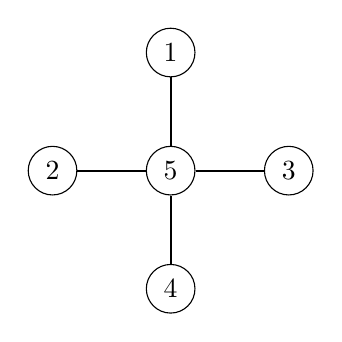
\begin{tikzpicture}[node distance=1.5cm,
    every node/.style={circle,draw,minimum size=0.6cm}]
    \node (5) {5};
    \node (1) [above of=5] {1};
    \node (2) [left of=5] {2};
    \node (3) [right of=5] {3};
    \node (4) [below of=5] {4};
    
    \draw[thick] (1) -- (5);
    \draw[thick] (2) -- (5);
    \draw[thick] (3) -- (5);
    \draw[thick] (4) -- (5);
\end{tikzpicture}
\end{center}

All peripheral nodes have \textbf{identical adjacency vectors}:
\begin{align*}
\bm{A}_1 = \bm{A}_2 = \bm{A}_3 = \bm{A}_4 = [0, 0, 0, 0, 1]
\end{align*}

\textbf{With only $\mathcal{L}_{2^{nd}}$:} All four peripheral nodes would collapse to a single point in the embedding space—a complete loss of structural information!

\textbf{With $\mathcal{L}_{2^{nd}} + \mathcal{L}_{1^{st}}$:} 
\begin{itemize}
    \item All peripheral nodes are forced close to the center (node 5)
    \item But they can maintain distinct positions around the center
    \item The embedding might look like points arranged in a circle around node 5
\end{itemize}

This demonstrates why \textbf{neither loss alone is sufficient}—we need both to capture the full graph structure.
\end{example}

\subsection{The Role of the Hyperparameter $\alpha$}

The balance between the two losses is controlled by $\alpha$ in:
\[
\mathcal{L}_{total} = \mathcal{L}_{2^{nd}} + \alpha \mathcal{L}_{1^{st}} + \lambda \mathcal{L}_{reg}
\]

\begin{itemize}
    \item \textbf{Small $\alpha$ (e.g., $10^{-6}$):} Emphasis on second-order proximity
    \begin{itemize}
        \item Nodes with similar neighborhoods cluster tightly
        \item Risk of collapsing embeddings for nodes with identical neighborhoods
        \item Good for capturing global community structure
    \end{itemize}
    \item \textbf{Large $\alpha$ (e.g., $10^{-2}$):} Emphasis on first-order proximity
    \begin{itemize}
        \item Direct connections strongly preserved
        \item Nodes with identical neighborhoods can be distinguished
        \item Good for preserving local graph topology
    \end{itemize}
    \item \textbf{Moderate $\alpha$ (e.g., $10^{-5}$):} Balanced approach
    \begin{itemize}
        \item Captures both local and global structure
        \item Typically the best choice in practice
    \end{itemize}
\end{itemize}

\begin{example}[Why We Need Both]
Consider a graph with two tightly-knit communities connected by a single edge:

\begin{center}
\begin{tikzpicture}[node distance=1cm,
    every node/.style={circle,draw,minimum size=0.6cm,font=\small}]
    % Community 1
    \node (1) {1};
    \node (2) [right of=1] {2};
    \node (3) [below of=1] {3};
    \node (4) [below of=2] {4};
    
    \draw[thick] (1) -- (2);
    \draw[thick] (1) -- (3);
    \draw[thick] (2) -- (4);
    \draw[thick] (3) -- (4);
    \draw[thick] (1) -- (4);
    \draw[thick] (2) -- (3);
    
    % Bridge
    \node (5) [right=2cm of 2] {5};
    \draw[thick,red] (2) -- (5);
    
    % Community 2
    \node (6) [right of=5] {6};
    \node (7) [below of=5] {7};
    \node (8) [below of=6] {8};
    
    \draw[thick] (5) -- (6);
    \draw[thick] (5) -- (7);
    \draw[thick] (6) -- (8);
    \draw[thick] (7) -- (8);
    \draw[thick] (5) -- (8);
    \draw[thick] (6) -- (7);
\end{tikzpicture}
\end{center}

\begin{itemize}
    \item \textbf{Only $\mathcal{L}_{2^{nd}}$}: Nodes 2 and 5 (connected by red edge) might be separated because they have very different neighborhoods
    \item \textbf{Only $\mathcal{L}_{1^{st}}$}: The model might miss that nodes 1,2,3,4 form a tight community
    \item \textbf{Both combined}: Preserves both the bridge connection and community structure
\end{itemize}
\end{example}

\section{Complete Worked Example}

Let's work through a complete example with a small graph.

\begin{example}[Complete SDNE Computation]
Consider the following 4-node graph:

\begin{center}
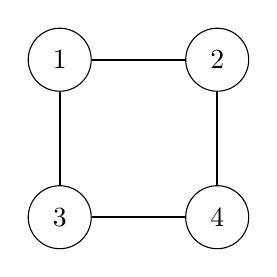
\begin{tikzpicture}[node distance=2cm,
    every node/.style={circle,draw,minimum size=0.8cm}]
    \node (1) {1};
    \node (2) [right of=1] {2};
    \node (3) [below of=1] {3};
    \node (4) [below of=2] {4};
    
    \draw[thick] (1) -- (2);
    \draw[thick] (1) -- (3);
    \draw[thick] (2) -- (4);
    \draw[thick] (3) -- (4);
\end{tikzpicture}
\end{center}

\textbf{Adjacency Matrix}:
\[
\bm{A} = \begin{bmatrix}
0 & 1 & 1 & 0 \\
1 & 0 & 0 & 1 \\
1 & 0 & 0 & 1 \\
0 & 1 & 1 & 0
\end{bmatrix}
\]

\textbf{Suppose} the encoder produces embeddings:
\begin{align*}
\bm{y}_1 &= [0.5, 0.5] \\
\bm{y}_2 &= [1.0, 0.5] \\
\bm{y}_3 &= [0.5, 1.0] \\
\bm{y}_4 &= [1.0, 1.0]
\end{align*}

And the decoder reconstructs:
\[
\tilde{\bm{A}} = \begin{bmatrix}
0.05 & 0.90 & 0.85 & 0.10 \\
0.90 & 0.05 & 0.10 & 0.92 \\
0.85 & 0.10 & 0.05 & 0.88 \\
0.10 & 0.92 & 0.88 & 0.05
\end{bmatrix}
\]

\subsection*{Computing $\mathcal{L}_{2^{nd}}$ (with $\beta = 5$)}

For node 1: $\bm{A}_1 = [0, 1, 1, 0]$, $\tilde{\bm{A}}_1 = [0.05, 0.90, 0.85, 0.10]$

Weight vector: $\bm{B}_1 = [1, 5, 5, 1]$

Error: $\bm{A}_1 - \tilde{\bm{A}}_1 = [-0.05, 0.10, 0.15, -0.10]$

Weighted error: $[-0.05, 0.50, 0.75, -0.10]$

Squared norm: $0.0025 + 0.25 + 0.5625 + 0.01 = 0.825$

Similarly computing for all nodes:
\begin{align*}
\mathcal{L}_{2^{nd}}(1) &= 0.825 \\
\mathcal{L}_{2^{nd}}(2) &= 0.845 \\
\mathcal{L}_{2^{nd}}(3) &= 0.870 \\
\mathcal{L}_{2^{nd}}(4) &= 0.850
\end{align*}

Total: $\mathcal{L}_{2^{nd}} = 3.39$

\subsection*{Computing $\mathcal{L}_{1^{st}}$}

The graph has edges: $(1,2), (1,3), (2,4), (3,4)$

\begin{align*}
\norm{\bm{y}_1 - \bm{y}_2}^2 &= \norm{[-0.5, 0]}^2 = 0.25 \\
\norm{\bm{y}_1 - \bm{y}_3}^2 &= \norm{[0, -0.5]}^2 = 0.25 \\
\norm{\bm{y}_2 - \bm{y}_4}^2 &= \norm{[0, -0.5]}^2 = 0.25 \\
\norm{\bm{y}_3 - \bm{y}_4}^2 &= \norm{[-0.5, 0]}^2 = 0.25
\end{align*}

Total: $\mathcal{L}_{1^{st}} = 0.25 + 0.25 + 0.25 + 0.25 = 1.0$

\subsection*{Computing Total Loss}

With $\alpha = 1$ and $\lambda = 0.001$, and assuming $\norm{\bm{W}}^2_F = 100$:

\begin{align*}
\mathcal{L}_{total} &= \mathcal{L}_{2^{nd}} + \alpha \mathcal{L}_{1^{st}} + \lambda \mathcal{L}_{reg} \\
&= 3.39 + 1 \cdot 1.0 + 0.001 \cdot 100 \\
&= 3.39 + 1.0 + 0.1 \\
&= 4.49
\end{align*}
\end{example}

\section{Training Procedure}

\subsection{Algorithm}

\begin{algorithm}
\caption{Training Graph Autoencoder (SDNE)}
\begin{algorithmic}[1]
\Require Graph adjacency matrix $\bm{A}$, embedding dimension $d$, hyperparameters $\alpha, \beta, \lambda$
\Ensure Node embeddings $\{\bm{y}_i\}_{i=1}^n$
\State Initialize encoder weights $\bm{W}^{enc}$ and decoder weights $\bm{W}^{dec}$
\For{epoch = 1 to $N_{epochs}$}
    \For{batch $\mathcal{B}$ of nodes}
        \State \textbf{Forward pass:}
        \State \quad Encode: $\bm{Y}_{\mathcal{B}} = f_{\bm{W}^{enc}}(\bm{A}_{\mathcal{B}})$ \Comment{Get embeddings}
        \State \quad Decode: $\tilde{\bm{A}}_{\mathcal{B}} = g_{\bm{W}^{dec}}(\bm{Y}_{\mathcal{B}})$ \Comment{Reconstruct adjacency}
        \State
        \State \textbf{Compute losses:}
        \State \quad $\mathcal{L}_{2^{nd}} = \sum_{i \in \mathcal{B}} \norm{(\tilde{\bm{A}}_i - \bm{A}_i) \hadamard \bm{B}_i}^2$
        \State \quad $\mathcal{L}_{1^{st}} = \sum_{i,j \in \mathcal{B}} A_{ij} \norm{\bm{y}_i - \bm{y}_j}^2$
        \State \quad $\mathcal{L}_{reg} = \norm{\bm{W}^{enc}}^2_F + \norm{\bm{W}^{dec}}^2_F$
        \State \quad $\mathcal{L}_{total} = \mathcal{L}_{2^{nd}} + \alpha \mathcal{L}_{1^{st}} + \lambda \mathcal{L}_{reg}$
        \State
        \State \textbf{Backward pass:}
        \State \quad Compute gradients: $\nabla_{\bm{W}^{enc}} \mathcal{L}_{total}$, $\nabla_{\bm{W}^{dec}} \mathcal{L}_{total}$
        \State \quad Update weights using optimizer (e.g., Adam)
    \EndFor
\EndFor
\State \Return Final embeddings $\{\bm{y}_i\}_{i=1}^n$
\end{algorithmic}
\end{algorithm}

\subsection{Computational Complexity}

\begin{itemize}
    \item \textbf{$\mathcal{L}_{2^{nd}}$}: $O(n \cdot m)$ where $m$ is average degree
    \item \textbf{$\mathcal{L}_{1^{st}}$}: $O(|E|)$ where $|E|$ is number of edges
    \item \textbf{Per iteration}: $O(n \cdot m + |E|)$
\end{itemize}

For large graphs, the input dimension (number of nodes) can be millions, making naive implementations infeasible. Solutions include:
\begin{itemize}
    \item Mini-batch training
    \item Sampling neighborhoods
    \item Using Graph Neural Networks (GNNs) instead
\end{itemize}

\section{Interpretation and Properties}

\subsection{What Does the Embedding Space Learn?}

The trained embeddings have several interesting properties:

\begin{proposition}[Community Detection]
Nodes in the same community (densely connected subgraph) will cluster together in the embedding space due to shared second-order proximity.
\end{proposition}

\begin{proposition}[Bridge Nodes]
Nodes that connect different communities will have embeddings positioned between the community clusters, preserving first-order connections to both sides.
\end{proposition}

\subsection{Visualization Example}

Consider the Karate Club graph (see Section \ref{graph-autoencoders:sec:karate_club}). After training SDNE with $d=2$, we can visualize the embeddings:

\begin{center}
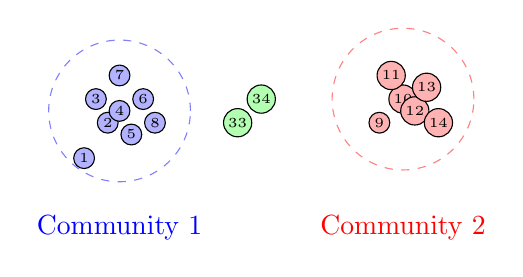
\begin{tikzpicture}[scale=1.5]
    % Community 1 (Instructor)
    \foreach \i/\x/\y in {1/0/0, 2/0.2/0.3, 3/0.1/0.5, 4/0.3/0.4, 5/0.4/0.2, 6/0.5/0.5, 7/0.3/0.7, 8/0.6/0.3} {
        \node[circle,fill=blue!30,draw,inner sep=1pt] at (\x,\y) {\tiny \i};
    }
    
    % Community 2 (Administrator)
    \foreach \i/\x/\y in {9/2.5/0.3, 10/2.7/0.5, 11/2.6/0.7, 12/2.8/0.4, 13/2.9/0.6, 14/3.0/0.3} {
        \node[circle,fill=red!30,draw,inner sep=1pt] at (\x,\y) {\tiny \i};
    }
    
    % Bridge nodes
    \node[circle,fill=green!30,draw,inner sep=1pt] at (1.5,0.5) {\tiny 34};
    \node[circle,fill=green!30,draw,inner sep=1pt] at (1.3,0.3) {\tiny 33};
    
    \draw[dashed,blue!50] (0.3,0.4) circle (0.6cm);
    \draw[dashed,red!50] (2.7,0.5) circle (0.6cm);
    
    \node[below,blue] at (0.3,-0.4) {Community 1};
    \node[below,red] at (2.7,-0.4) {Community 2};
\end{tikzpicture}
\end{center}

The embedding space preserves:
\begin{itemize}
    \item Community structure (blue and red clusters)
    \item Bridge connections (green nodes in between)
    \item Local neighborhood similarity
\end{itemize}

\section{The Karate Club Graph}
\label{graph-autoencoders:sec:karate_club}

\subsection{Historical Context}

The Zachary's Karate Club graph is one of the most famous datasets in network science. It was collected by anthropologist Wayne Zachary in the 1970s during a study of a university karate club.

\begin{tcolorbox}[colback=orange!5!white,colframe=orange!75!black,title=The Story]
Zachary observed social interactions between 34 members of a karate club over a period of 3 years (1970-1972). During this time, a conflict arose between the club's instructor (Mr. Hi) and the club's administrator (John A.) over various issues including the instructor's pricing policies.

This conflict eventually led to a split of the club into two separate organizations. Remarkably, Zachary found that the eventual split could be accurately predicted from the network structure of social ties using community detection algorithms—even before the split actually occurred!
\end{tcolorbox}

\subsection{Graph Properties}

\begin{itemize}
    \item \textbf{Nodes}: 34 (club members)
    \item \textbf{Edges}: 78 (social interactions outside of club activities, such as socializing at bars and attending karate tournaments together)
    \item \textbf{Two main communities}: 
    \begin{itemize}
        \item Instructor's faction (loyal to Mr. Hi)
        \item Administrator's faction (loyal to John A.)
    \end{itemize}
    \item \textbf{Bridge nodes}: Members with connections to both factions who faced difficult decisions during the split
\end{itemize}

\subsection{Why It's Important}

The Karate Club graph has become a standard benchmark in network science because:

\begin{enumerate}
    \item \textbf{Real-world validation}: The network structure predicted the actual social split with high accuracy
    \item \textbf{Clear community structure}: It exhibits two well-defined communities with some inter-community connections
    \item \textbf{Manageable size}: With only 34 nodes, it's small enough to visualize completely and understand intuitively
    \item \textbf{Complex enough}: Despite its size, it demonstrates important phenomena like community detection, bridge nodes, and the predictive power of network analysis
    \item \textbf{Historical significance}: It's one of the earliest examples of using network analysis to understand and predict social phenomena
\end{enumerate}

The Karate Club graph is now a standard benchmark for:
\begin{itemize}
    \item Community detection algorithms
    \item Graph embedding methods
    \item Social network analysis techniques
    \item Network visualization approaches
\end{itemize}

\section{Practical Implementation}

\subsection{Python Implementation Snippet}

Here's how you can use SDNE in practice with the GEM library:

\begin{verbatim}
import networkx as nx
from gem.embedding.sdne import SDNE

# Load Karate Club graph
G = nx.karate_club_graph()

# Initialize SDNE
sdne = SDNE(
    d=2,                # embedding dimension
    beta=5,             # edge weight for reconstruction
    alpha=1e-5,         # first-order loss weight
    nu1=1e-6,           # L1 regularization
    nu2=1e-6,           # L2 regularization
    K=3,                # number of layers
    n_units=[50, 15],   # hidden layer sizes
    rho=0.3,            # corruption level for denoising
    n_iter=10,          # number of iterations
    xeta=0.01,          # learning rate
    n_batch=100         # batch size
)

# Learn embeddings
sdne.learn_embedding(G)
embeddings = sdne.get_embedding()

# embeddings is now a dict: node_id -> embedding_vector
\end{verbatim}

\subsection{Hyperparameter Tuning}

\begin{table}[h]
\centering
\begin{tabular}{@{}lll@{}}
\toprule
\textbf{Parameter} & \textbf{Typical Range} & \textbf{Effect} \\ \midrule
$\beta$ & 5-10 & Higher = more focus on edge reconstruction \\
$\alpha$ & $10^{-5}$ to $10^{-2}$ & Higher = more first-order preservation \\
$\lambda$ & $10^{-6}$ to $10^{-4}$ & Higher = more regularization \\
$d$ & 2-128 & Embedding dimension \\
layers & 2-4 & Deeper = more expressive (but harder to train) \\ \bottomrule
\end{tabular}
\caption{Typical hyperparameter ranges for SDNE}
\end{table}

\section{Advantages and Limitations}

\subsection{Advantages}

\begin{itemize}
    \item \textbf{Preserves both local and global structure} through combined loss
    \item \textbf{Handles weighted graphs} naturally via $S_{ij}$
    \item \textbf{Non-linear embeddings} capture complex relationships
    \item \textbf{End-to-end differentiable} enables gradient-based optimization
\end{itemize}

\subsection{Limitations}

\begin{itemize}
    \item \textbf{Scalability}: Input dimension equals number of nodes (problematic for large graphs)
    \item \textbf{Transductive}: Cannot directly embed new nodes without retraining
    \item \textbf{No node features}: Only uses graph structure (though can be extended)
    \item \textbf{Hyperparameter sensitivity}: Requires careful tuning of $\alpha$, $\beta$, $\lambda$
\end{itemize}

\subsection{When to Use SDNE}

Use SDNE when:
\begin{itemize}
    \item Graph has $<100,000$ nodes
    \item Need to preserve both community structure and local connections
    \item Have computational resources for training
    \item Don't need to embed new nodes after training
\end{itemize}

Consider alternatives when:
\begin{itemize}
    \item Graph is very large ($>1$ million nodes) $\rightarrow$ use sampling-based methods (DeepWalk, Node2Vec)
    \item Need inductive capability $\rightarrow$ use GNNs (GraphSAGE, GAT)
    \item Have rich node features $\rightarrow$ use feature-aware methods
\end{itemize}

\section{Extensions and Related Methods}

\subsection{Variational Graph Autoencoders (VGAE)}

Replace deterministic encoder with variational encoder:
\begin{itemize}
    \item Encoder outputs mean $\bm{\mu}_i$ and variance $\bm{\sigma}_i^2$
    \item Sample: $\bm{y}_i \sim \mathcal{N}(\bm{\mu}_i, \bm{\sigma}_i^2)$
    \item Add KL divergence term to loss
\end{itemize}

Benefits: Better generalization, uncertainty quantification

\subsection{Graph Attention Autoencoders}

Incorporate attention mechanisms to weight neighborhood importance:
\[
\bm{y}_i = \sum_{j \in \mathcal{N}(i)} \alpha_{ij} \bm{h}_j
\]
where $\alpha_{ij}$ are learned attention weights.

\subsection{Deep Graph Infomax}

Maximize mutual information between local and global graph representations instead of reconstruction.

\section{Conclusion}

Graph autoencoders provide a powerful framework for learning node embeddings by:
\begin{enumerate}
    \item Using weighted reconstruction loss ($\mathcal{L}_{2^{nd}}$) to handle graph sparsity
    \item Explicitly preserving direct connections ($\mathcal{L}_{1^{st}}$)
    \item Combining both to capture multi-scale graph structure
\end{enumerate}

The key innovation of SDNE is recognizing that standard reconstruction error fails for graphs and designing loss functions that account for the asymmetric information content of edges versus non-edges.

\subsection{Key Takeaways}

\begin{tcolorbox}[colback=purple!5!white,colframe=purple!75!black,title=Summary]
\begin{itemize}
    \item \textbf{$\beta$-weighting} addresses sparse graph reconstruction by penalizing edge errors more heavily
    \item \textbf{Second-order proximity} ($\mathcal{L}_{2^{nd}}$) preserves community structure and neighborhood similarity
    \item \textbf{First-order proximity} ($\mathcal{L}_{1^{st}}$) preserves direct connections between nodes
    \item \textbf{Combined loss} captures multi-scale structure (local and global)
    \item \textbf{Scalability} remains a challenge for very large graphs (millions of nodes)
\end{itemize}
\end{tcolorbox}

\section*{Further Reading}

\begin{itemize}
    \item Wang, D., Cui, P., \& Zhu, W. (2016). Structural deep network embedding. \textit{KDD}.
    \item Kipf, T. N., \& Welling, M. (2016). Variational graph auto-encoders. \textit{NIPS Workshop}.
    \item Hamilton, W. L. (2020). \textit{Graph representation learning}. Synthesis Lectures on AI and ML.
    \item Zachary, W. W. (1977). An information flow model for conflict and fission in small groups. \textit{Journal of Anthropological Research}, 33(4), 452-473.
\end{itemize}
\end{notechapter}
